% Metódy inžinierskej práce

\documentclass[10pt,twoside,slovak,a4paper,oneside]{article}

\usepackage[slovak]{babel}
%\usepackage[T1]{fontenc}
\usepackage[IL2]{fontenc} % lepšia sadzba písmena Ľ než v T1
\usepackage[utf8]{inputenc}
\usepackage{graphicx}
\usepackage{url} % príkaz \url na formátovanie URL
\usepackage{hyperref} % odkazy v texte budú aktívne (pri niektorých triedach dokumentov spôsobuje posun textu)
\usepackage{cite}
%\usepackage{times}
\usepackage[nomarginpar, margin=1.7in]{geometry}%margin inconsistency


\pagestyle{headings}

\title{Agilné postupy pri vývoji medicínskeho softvéru\thanks{Semestrálny projekt v predmete Metódy inžinierskej práce, ak. rok 2021/22, vedenie: Ing. Vladimír Mlynarovič PhD.}} 

\author{Irina Makarova\\[2pt]
	{\small Slovenská technická univerzita v Bratislave}\\
	{\small Fakulta informatiky a informačných technológií}\\
	{\small \texttt{xmakarovai@stuba.sk}}
	}

%\date{\small 4. oktober 2021}



\begin{document}
\renewcommand{\abstractname}{\vspace{-\baselineskip}} %removes abstract heading
\maketitle

\begin{abstract}
V súčasnosti sa rýchlo vyvíja trh zdravotníckych prenositeľných zariadení. Vodopádový model, ktorý sa klasicky používal pri vývoji bezpečnostne kritického softvéru, už pre svoju zdĺhavosť a nepružnosť nepredstavuje optimálny postup. Do popredia sa dostávajú rôzne agilné a kombinované prístupy, čo prináša so sebou otázku, ako implementovať do procesu vývoja agilné metódy a pri tom dodržať požadované normy. Tento článok prináša stručný prehľad aktuálne platných noriem; vysvetľuje podstatu vodopádového a agilných modelov (Scrum, XP, DSDM), porovnáva ich a poukazuje na črty jednotlivých stratégií, ktoré sú prínosné pre túto oblasť. V článku sa uvádzajú niektoré existujúce riešenia, ako sa tieto modely dajú efektívne kombinovať pri vývoji medicínskeho softvéru.
\end{abstract}

\section{Úvod} 


skuska citovania\cite{mccaffery2019}

\section{Predpisy o zdravotníckych pomôckach}
European Medical Device Regulation 2017/745 (MDR): za zdravotnícku pomôcku sa považuje akýkoľvek výrobok, ktorý je výrobcom určený na použitie za účelom/mi ako sú diagnostika, predikcia, sledovanie, prevencia, liečba alebo zmiernenie choroby a ktorý nedosahuje svoj účinok pomocou farmakologických alebo imunologických prostriedkov. Pod túto definíciu spadá nielen softvér zabudovaný v špecializovaných prístrojoch, ale aj softvér ako taký, ak je určený na lekárske účely, tzv. SaMD. Podľa FDA existujú tri bezpečnostné triedy zdravotníckych pomôcok; europska klasifikácia je veľmi podobná. Pomôcky triedy I nie sú určené na udržiavanie ľudského života a nesmú predstavovať riziko poškodenia zdravia (napr. teplomer). Pomôcky triedy II by v prípade zlyhania mohli používateľom ublížiť. Zdravotnícke pomôcky triedy III sú zvyčajne pomôcky, ktoré podporujú alebo udržujú ľudský život (implantovateľný kardiostimulátor).
Kľúčovým štandardom pre vývojárov medicínskeho softvéru je ISO IEC 62304:2006.

\section{Modely vývoja softvéru}
Pri tradičnom, sekvenčnom vývoji softvéru sa najprv zostavuje dokument všetkých požiadaviek na softvérový produkt. Následne sa produkt na základe týchto požiadaviek navrhuje a implemetuje. Často sa však stáva, že požiadavky, ktoré zadá zákazník sú nepresné a neúplné, preto sa treba vracať k počiatočným fázam vývoja. V dôsledku zmien požiadaviek sa potom musí zvýšiť rozpočet alebo oddialiť termín dodania. 
Pri klasickom vývoji softvéru je funkcionalita systému pevne stanovená a zdroje a čas potrebný na dokončenie projektu, sa menia. V agilných metódach je to naopak - prostriedky a čas sú fixne stanovené a mení sa funkcionalita softvéru na základe požiadaviek od používateľa.
\subsection{V-model}

%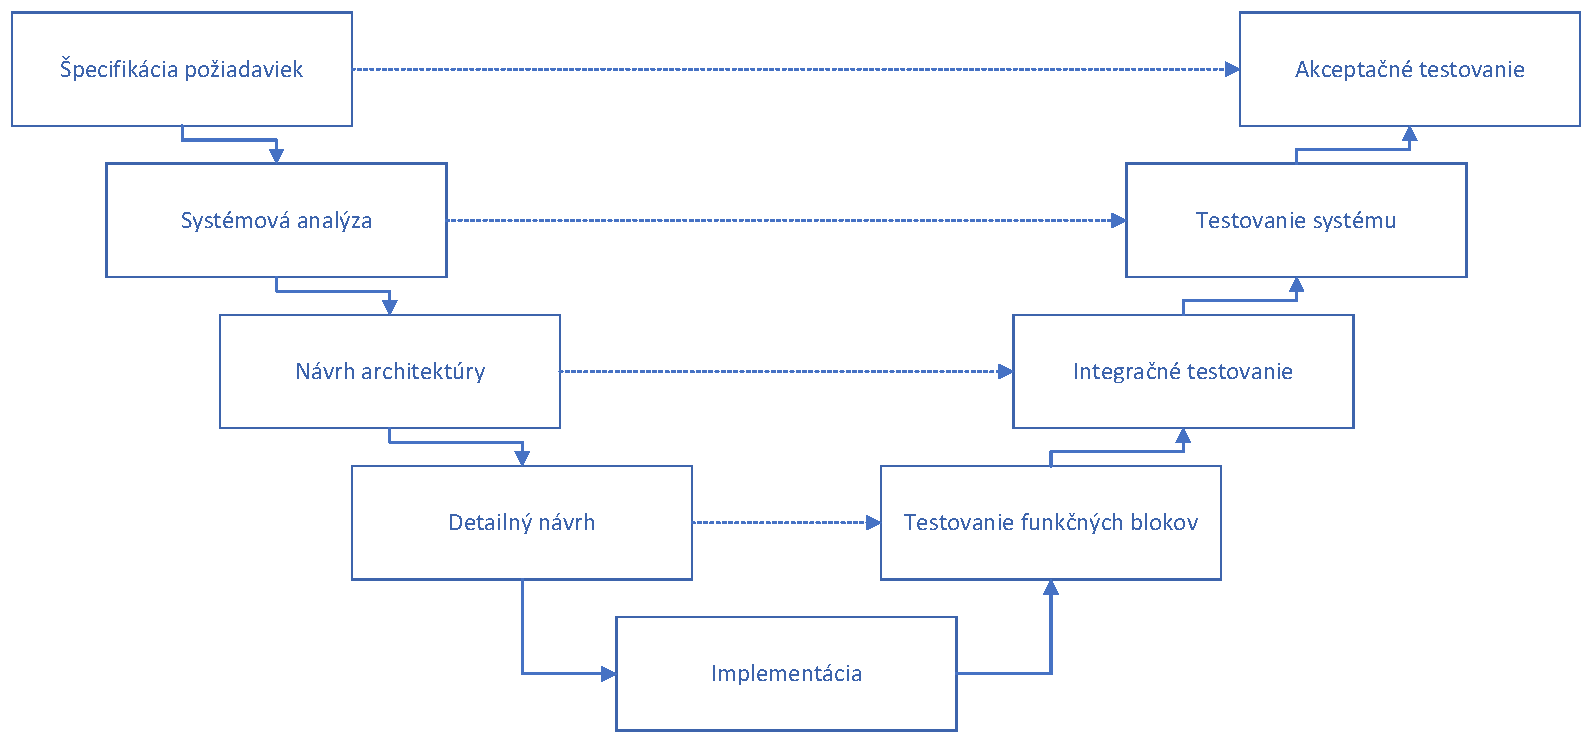
\includegraphics[width=1\textwidth]{V.pdf}

\subsection{Agilné metódy}
Spoločné vlastnosti agilných rámcov a metodík:
\begin{itemize}
\item Zákazník (používateľ) je zainteresovaný do procesu vývoja
\item Iteratívny a inkrementálny spôsob vývoja 
\item Rýchla odozva na zmeny požiadaviek
\item Časté testovanie
\end{itemize}
Na konci každého cyklu vzniká funkčná verzia produktu. Pravidelné dodávky v krátkych iteráciách umožňujú priebežne riadiť požiadavky a prispôsobenie sa trhu. 
Manifest pre agilný vývoj softvéru

\paragraph{Scrum}je rámec, ktorý umožňuje riešiť komplexné adaptívne problémy a zároveň produktívne a kreatívne vytvárať produkty s najvyššou možnou hodnotou. Scrum je: 
\begin{itemize}
\item  ľahký,
\item jednoduchý na pochopenie a
\item ťažko zvládnuteľný
\end{itemize}
Tímy pracujúce podľa Scrum sú samo-organizované. Prácu vývojárskeho tímu usmerňuje scrum master, ktorý slúži ako styčný bod medzi ním a reprezentantom zákazníka. Scrum je založený aj na princípe ohraničenia času (time-boxing), pričom všetky aktivity - či už denné porady, sprint-y alebo akékoľvek rozhodnutia majú pevne obmedzenú časovú dĺžku. Toto obmedzenie slúži na zvýšenie produktivity, keďže nedáva tímu priestor na riešenie nepodstatných záležitostí. 

\paragraph{Extrémne programovanie}je postavené na piatich základoch: jednoduchosť, komunikácia, spätná väzba, rešpekt, odvaha.
\emph{Jednoduchost} – zameranie sa na hlavne to čo musí byť teraz vykonané; nesnazit sa urobiť to, čo by zákazník mohol chcieť implementovat neskôr.
\emph{Spätná väzba} – zákazník je aktívne zapojený do procesu vývoja. Na konci každej iterácie vzniká testovateľná funkcionalita. Vyvoj je riadeny testami. 
\emph{Komunikácia a rešpekt} – metodika predpoklada priaznive podmineky pre spoluprácu, vývojári by fyzicky mali byť na jednom mieste; spolocne vlastnenie kodu, keďže na jeho písaní sa podieľa celý tím; programovanie v paroch.
\paragraph{Metóda dynamického vývoja systémov}presne definuje postupy a pravidlá vývoja softvéru. Je založená na deviatich princípoch, ktoré by mali byť dodržiavané počas jednotlivých fáz životného cyklu. Vývoj sa riadi tak, aby bol ukončený do stanoveného času a za stanovené prostriedky. DSDM sa menej zaoberá programovacimi prístumi, ale podporuje skôr riadenie projektov. Dá sa kombinovať s inými agilnými metodikami.

\section{Kombinované prístupy}


\section{Záver}


% generuje zoznam literatúry z obsahu súboru literatura.bib
\bibliography{literatura}
\bibliographystyle{plain} % alpha/ abbrv/ plain
\end{document}
